\documentclass[a4paper,12pt]{article}
\usepackage[russian]{babel}
\usepackage[T2A]{fontenc}
\usepackage[utf8]{inputenc}
\usepackage[russian]{babel}
\usepackage{geometry}
\usepackage{amsmath}
\usepackage{graphicx}
\usepackage{cancel}
\usepackage{float} 
\usepackage{xcolor}
\usepackage{listings}
\usepackage{hyperref}
\usepackage{array}
\usepackage{caption}
\usepackage{booktabs}
\usepackage{amssymb}
\usepackage{subcaption}
\usepackage{caption}
\captionsetup[figure]{name=Рисунок}
\captionsetup[table]{name=Таблица}
\usepackage{pgfplots}
\pgfplotsset{compat=1.18}
\usetikzlibrary{arrows.meta}
\usepackage{capt-of}
\usepackage{multirow}
\usepackage[siunitx]{circuitikz}
\usepackage[bottom]{footmisc}
\usepackage{tcolorbox}
\usepackage{nicematrix}
\usepackage{tikz}
\usepackage{amssymb}

\usetikzlibrary{arrows.meta, matrix}
\lstset{
	language=Matlab,
	basicstyle=\ttfamily\small,
	keywordstyle=\color{blue}\bfseries,
	commentstyle=\color{gray}\itshape,
	stringstyle=\color{red},
	numberstyle=\tiny\color{gray},
	numbers=left,
	stepnumber=1,
	numbersep=8pt,
	backgroundcolor=\color{white},
	frame=single,
	breaklines=true,
	breakatwhitespace=true,
	tabsize=4,
	showspaces=false,
	showstringspaces=false,
	captionpos=b,
	escapeinside={\%*}{*)},
}
\geometry{left=1.5cm, right=2cm, bottom=2cm, top=2cm}

\begin{document}
	
	\begin{titlepage}
		\centering
		
		\vspace*{0.5cm}
		{\small
			Министерство науки и высшего образования Российской Федерации\\[2pt]
			Федеральное государственное автономное образовательное учреждение\\
			высшего образования\\[2pt]
			\textbf{«Национальный исследовательский университет ИТМО»}\\
		}
		
		\vspace{0.8cm}
		\hrule height 0.8pt
		\vspace{0.3cm}
		
		{\large Факультет систем управления и робототехники}
		
		\vspace{0.3cm}
		\hrule height 0.4pt
		\vspace{2.5cm}
		
		{\Huge\bfseries ОТЧЁТ}\\[0.4cm]
		{\LARGE\bfseries о лабораторной работе}\\[0.8cm]
		
		\begin{tcolorbox}[
			colback=gray!4,
			colframe=gray!10,
			boxrule=0.8pt,
			arc=4pt,
			left=12pt, right=12pt, top=8pt, bottom=8pt
			]
			\centering
			{\large По дисциплине:\\[4pt]}
			{\large\bfseries «Электронные устройства систем управления»}\\[10pt]
			{\large Тема:\\[4pt]}
			{\large\bfseries «Операционный усилитель в специализированных схемах»} \\[10pt]
			{\large Вариант: 6}
		\end{tcolorbox}
		
		\vspace{3cm}
		
		\begin{minipage}{0.45\textwidth}
			\raggedright
			{\large\bfseries Студенты:}\\[4pt]
				Охрименко Е. \\
				Шишкина М. \\
				Чупрова Д. \\
		\end{minipage}
		\hfill
		\begin{minipage}{0.45\textwidth}
			\raggedleft
			{\large\bfseries Преподаватели:}\\[4pt]
			Власов С. М. \\
			Зарина О. А.
		\end{minipage}
		
		\vfill
		\vspace{0.4cm}
		{\large Санкт-Петербург, 2026}
	\end{titlepage}
	
	\newpage
	\tableofcontents
	
\newpage
\section{Исследование нуль-компаратора}

Схема нуль-компаратора собрана на ОУ AD795, $R_1 = 10$ кОм, питание $\pm 12$ В.

\begin{figure}[H]
	\centering
	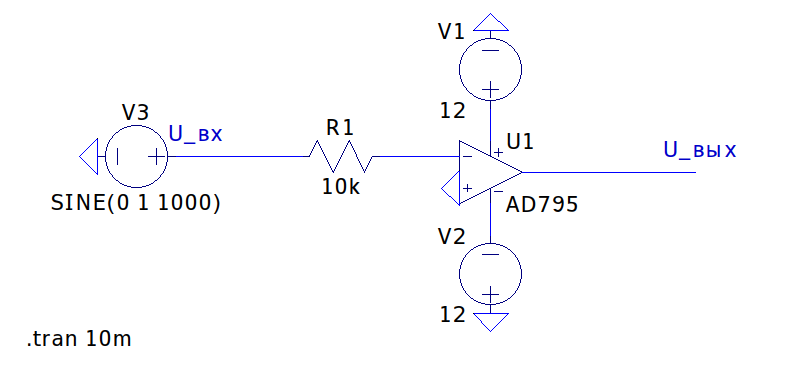
\includegraphics[width=0.7\textwidth]{../images/task1/NullComparatorScheme.png}
	\caption{Нуль-компаратор}
\end{figure}

При $U_{вх} = 1$ мВ ОУ работает в линейном режиме, выходной сигнал повторяет входной.

\begin{figure}[H]
	\centering
	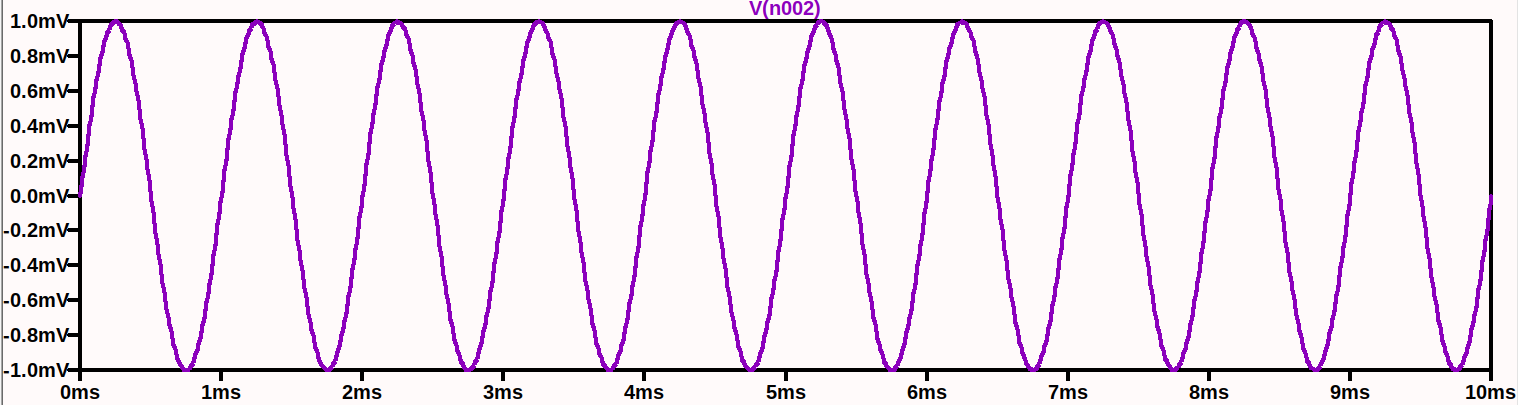
\includegraphics[width=1\textwidth]{../images/task1/1mInput.png}
	\caption{Входной сигнал, $U_{вх} = 1$ мВ}
\end{figure}

\begin{figure}[H]
	\centering
	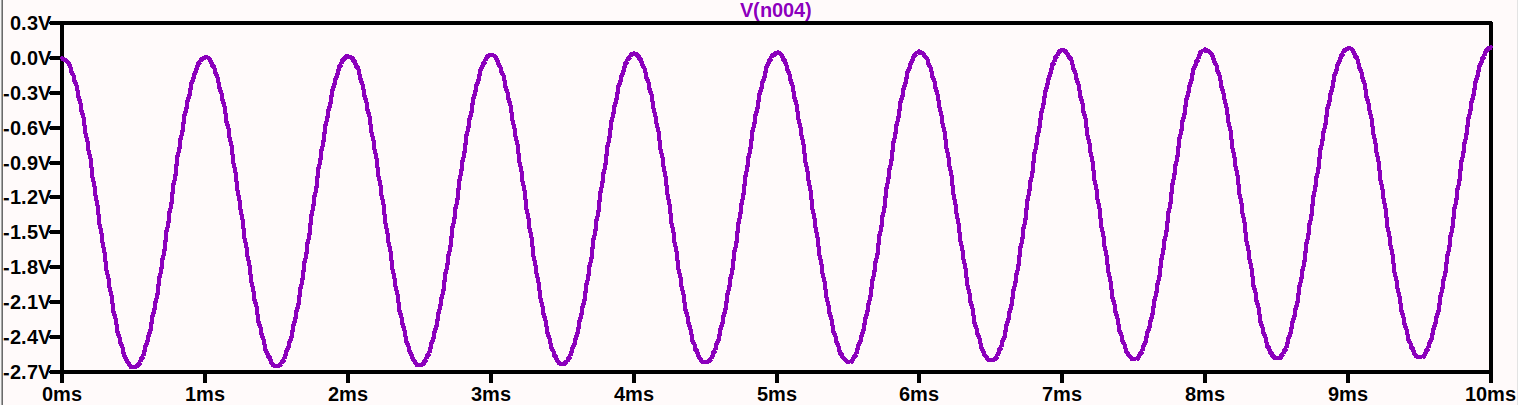
\includegraphics[width=1\textwidth]{../images/task1/1mOutput.png}
	\caption{Выходной сигнал, $U_{вх} = 1$ мВ}
\end{figure}

При $U_{вх} = 1$ В на выходе формируется прямоугольный сигнал $\approx \pm 9.5$ В.

\begin{figure}[H]
	\centering
	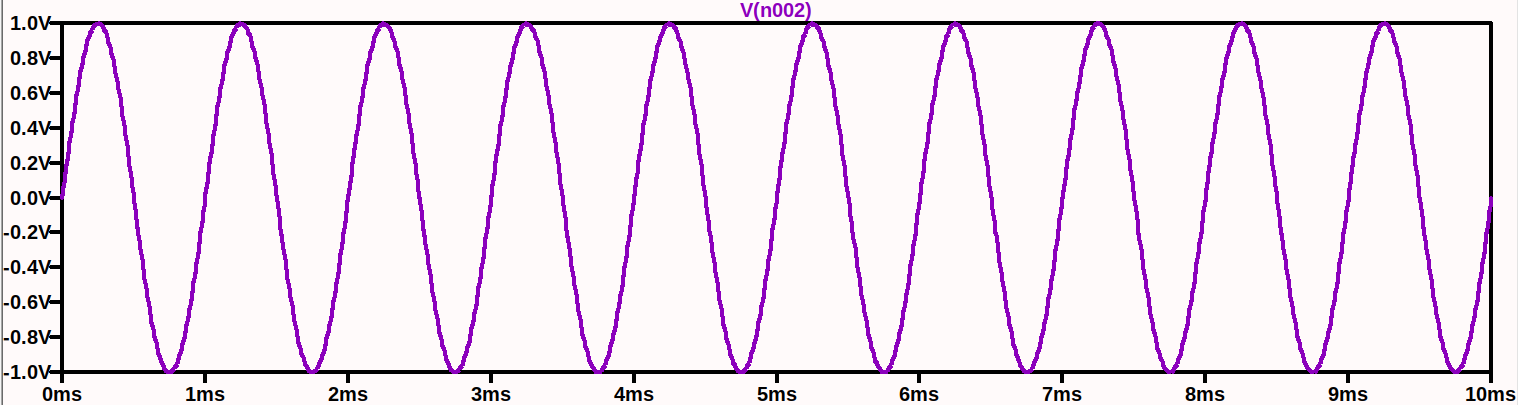
\includegraphics[width=1\textwidth]{../images/task1/1Input.png}
	\caption{Входной сигнал, $U_{вх} = 1$ В}
\end{figure}

\begin{figure}[H]
	\centering
	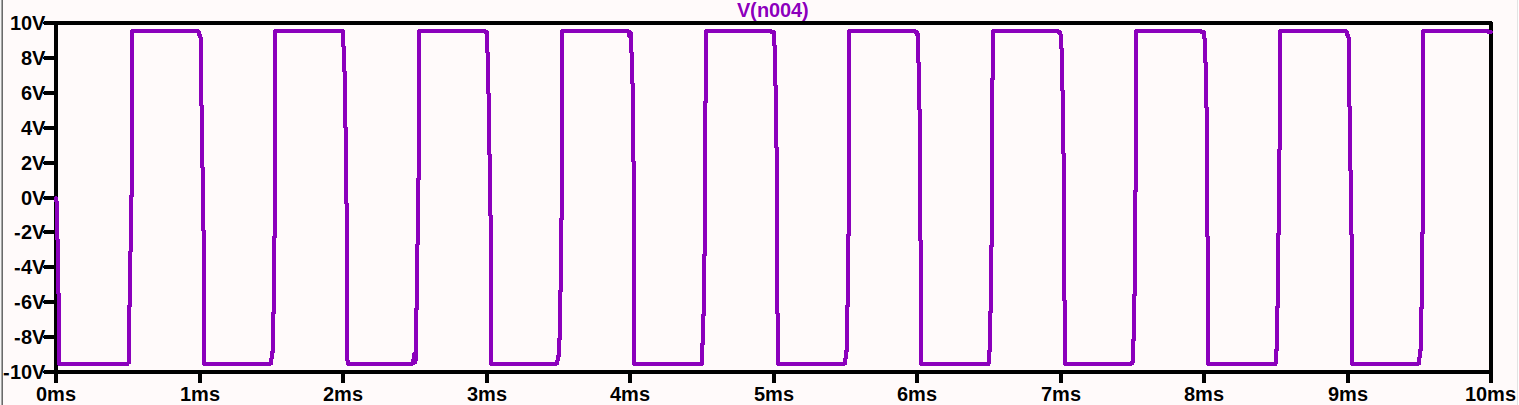
\includegraphics[width=1\textwidth]{../images/task1/1Output.png}
	\caption{Выходной сигнал, $U_{вх} = 1$ В}
\end{figure}

\textbf{Вывод:} Пороговое напряжение компаратора:
\[
U_\text{порог} = \frac{U_\text{нас}}{K} = \frac{10}{10^4} = 1 \text{ мВ}
\]
При $U_{вх} = 1$ мВ $\approx U_{порог}$ ОУ работает в линейном режиме — 
выходной сигнал повторяет форму входного. При $U_{вх} = 1$ В $\gg U_{порог}$ 
компаратор переключается при каждом переходе через ноль, формируя 
прямоугольный сигнал на выходе.

\newpage
\section{Исследование одновходового компаратора}

Схема одновходового компаратора собрана на ОУ AD795, питание $\pm 12$ В,
$U_{оп} = 10$ В, $R_1 = 100$ Ом.

Расчёт сопротивлений из условия $U_{пор} = -6$ В:
\[
R_2 = -U_{оп} \frac{R_1}{U_{пор}} = -10 \cdot \frac{100}{-6} \approx 167 \text{ Ом}
\]
\[
R_3 = \frac{R_1 \cdot R_2}{R_1 + R_2} = \frac{100 \cdot 167}{100 + 167} \approx 67 \text{ Ом}
\]

\begin{figure}[H]
	\centering
	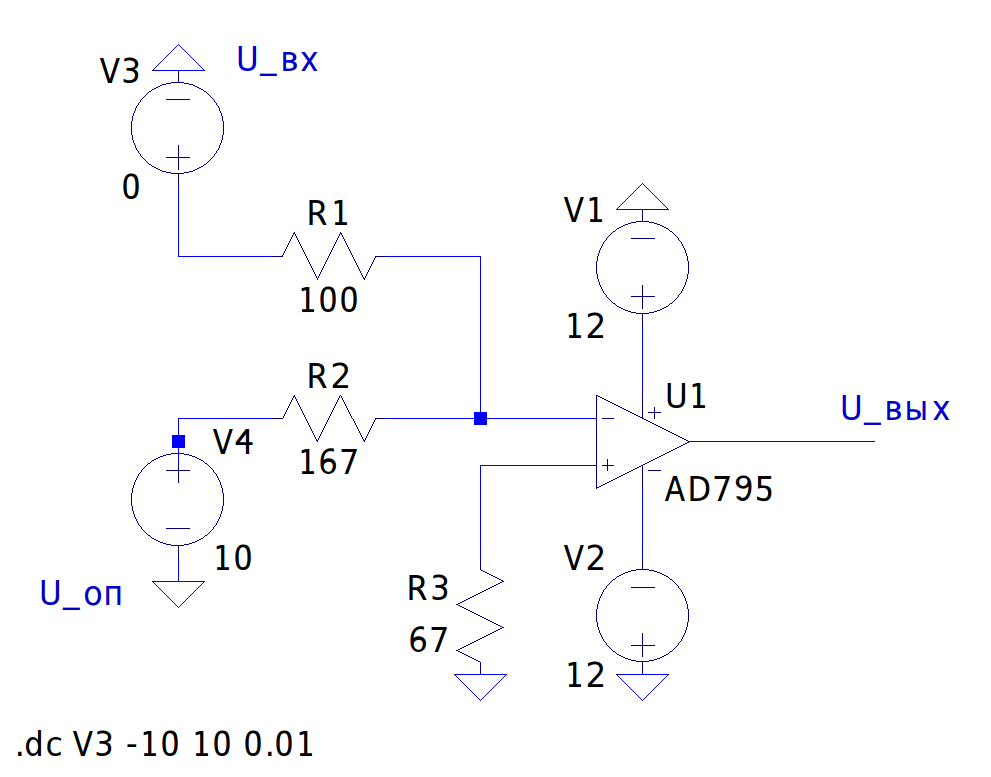
\includegraphics[width=0.7\textwidth]{../images/task2/singleInputComparator.png}
	\caption{Одновходовый компаратор}
\end{figure}

\begin{figure}[H]
	\centering
	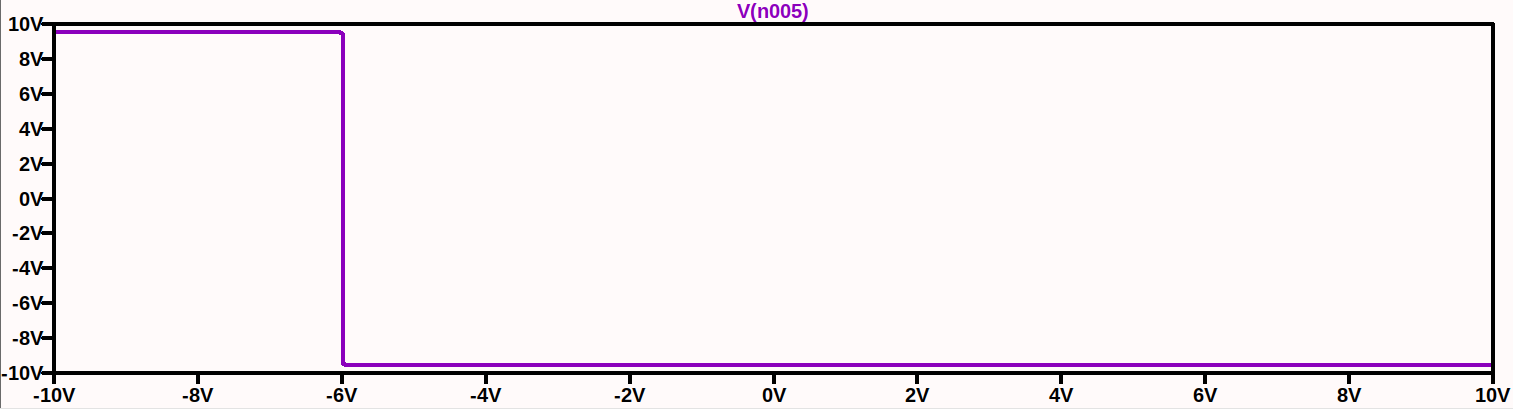
\includegraphics[width=1\textwidth]{../images/task2/transfer.png}
	\caption{Передаточная характеристика $U_{вых} = f(U_{вх})$}
\end{figure}

\textbf{Вывод:} при $U_{вх} < U_{пор} = -6$ В выход принимает значение 
$+U_{нас} \approx +9{,}5$ В, при $U_{вх} > U_{пор}$ — $-U_{нас} \approx -9{,}5$ В.
Компаратор корректно сравнивает входной сигнал с пороговым напряжением.

\newpage
\section{Исследование двухвходового компаратора}

Схема двухвходового компаратора собрана на ОУ AD795, питание $\pm 12$ В,
$U_{\text{оп}} = -1$ В, $R_1 = R_2 = 10$ кОм.

Пороговое напряжение определяется делителем $R_1$, $R_2$:
\[
U_{\text{пор}} = U_{\text{оп}} \cdot \frac{R_1}{R_1 + R_2} = -1 \cdot \frac{10}{10 + 10} = -0{,}5 \text{ В}
\]


\begin{figure}[H]
	\centering
	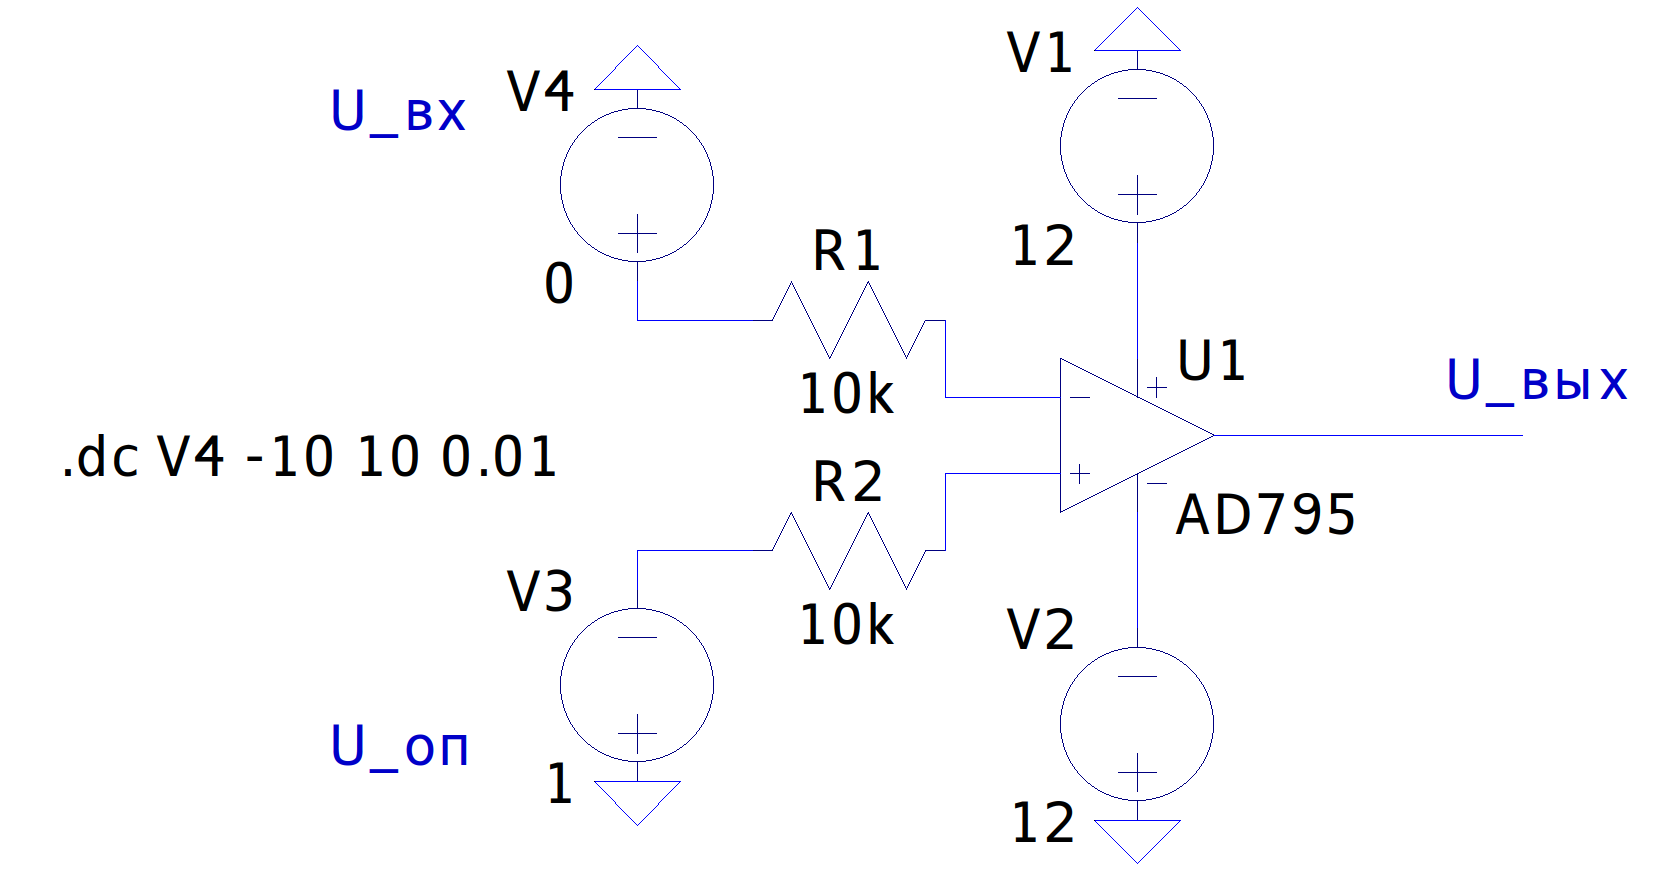
\includegraphics[width=0.7\textwidth]{../images/task3/twoComparatorScheme.png}
	\caption{Двухвходовый компаратор}
\end{figure}

\begin{figure}[H]
	\centering
	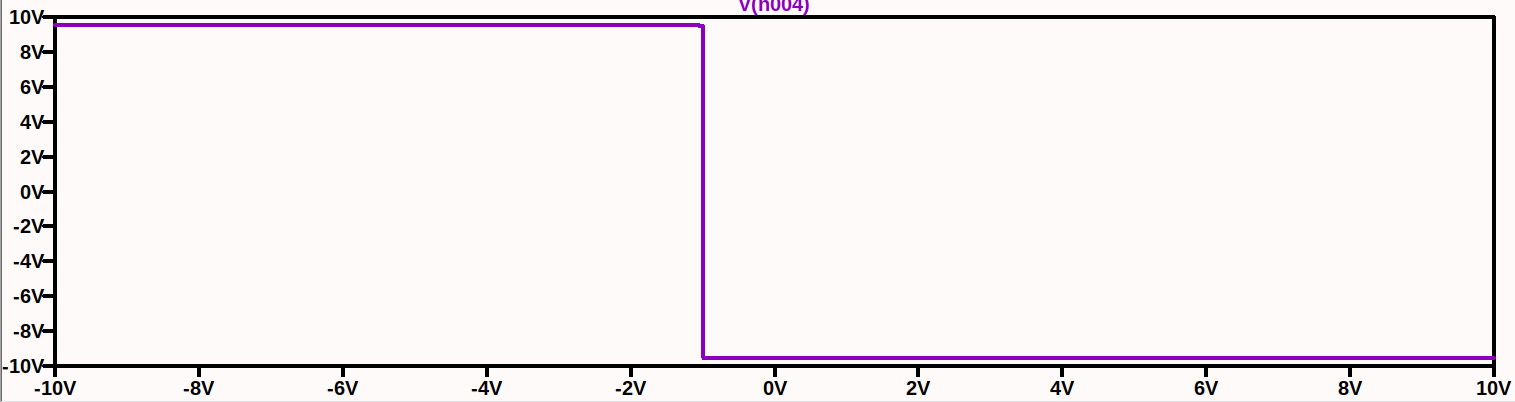
\includegraphics[width=1\textwidth]{../images/task3/twoInputComparator.png}
	\caption{Передаточная характеристика $U_{\text{вых}} = f(U_{\text{вх}})$}
\end{figure}

\textbf{Вывод:} при $U_{\text{вх}} < U_{\text{пор}} = -0{,}5$ В выход принимает значение
$+U_{\text{нас}} \approx +9{,}5$ В, при $U_{\text{вх}} > U_{\text{пор}}$ — $-U_{\text{нас}} \approx -9{,}5$ В.
Двухвходовый компаратор позволяет сравнивать входной сигнал с произвольным
опорным напряжением.


\newpage
\section{Исследование двухвходового компаратора с гистерезисом}

Схема двухвходового компаратора с гистерезисом собрана на ОУ AD795,
питание $\pm 12$ В, $U_{\text{оп}} = -1$ В, $R_1 = 1{,}1$ кОм, $R_2 = 10$ кОм,
$R_3 = 10$ кОм.

Расчёт напряжений:
\[
U_{\text{ВТО}} = U_{\text{оп}} \cdot \frac{R_2}{R_1+R_2} + \frac{R_1}{R_1+R_2} \cdot U_{\text{нас}}^+
= -1 \cdot \frac{10}{11{,}1} + \frac{1{,}1}{11{,}1} \cdot 11 \approx 2{,}5 \text{ В}
\]
\[
U_{\text{НТО}} = U_{\text{оп}} \cdot \frac{R_2}{R_1+R_2} - \frac{R_1}{R_1+R_2} \cdot U_{\text{нас}}^-
= -1 \cdot \frac{10}{11{,}1} - \frac{1{,}1}{11{,}1} \cdot 11 \approx 5{,}0 \text{ В}
\]
\[
\Delta U = 2 \cdot \frac{R_1}{R_1+R_2} \cdot U_{\text{нас}}^+
= 2 \cdot \frac{1{,}1}{11{,}1} \cdot 11 \approx 2{,}18 \text{ В}
\]

\begin{figure}[H]
	\centering
	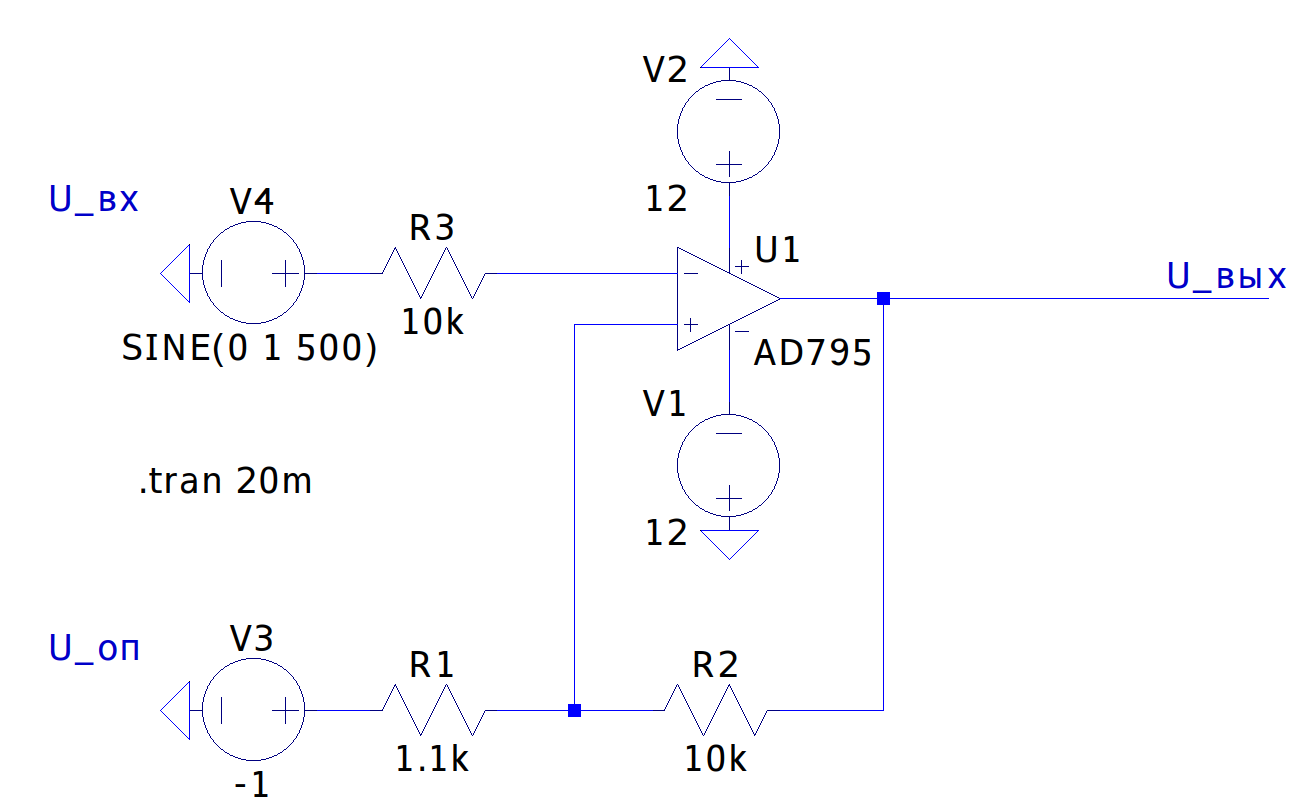
\includegraphics[width=0.7\textwidth]{../images/task4/chema4.png}
	\caption{Двухвходовый компаратор с гистерезисом}
\end{figure}

\begin{figure}[H]
	\centering
	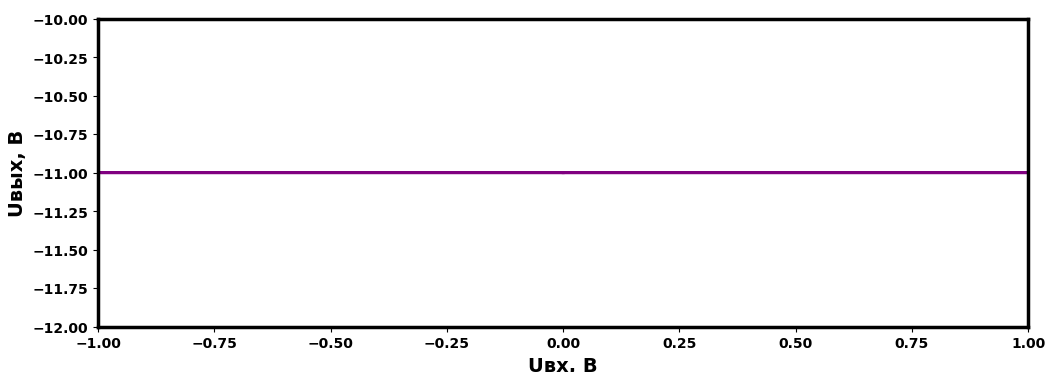
\includegraphics[width=1\textwidth]{../images/task4/line.png}
	\caption{Передаточная характеристика при малом сигнале}
\end{figure}

\begin{figure}[H]
	\centering
	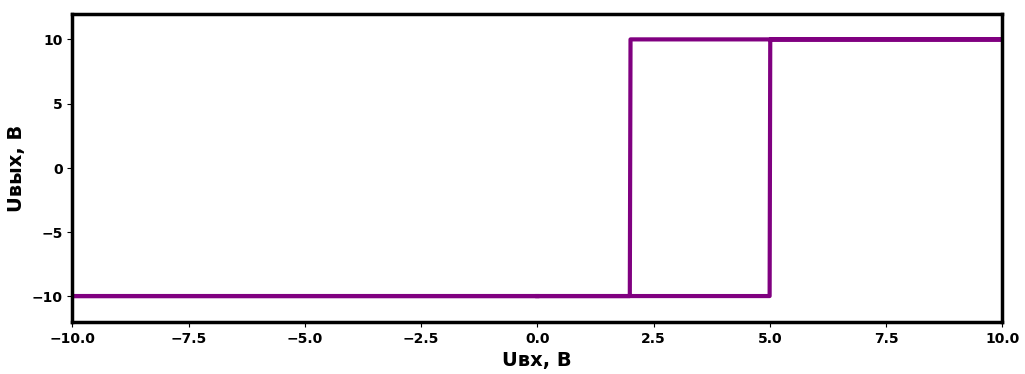
\includegraphics[width=1\textwidth]{../images/task4/hist.png}
	\caption{Передаточная характеристика $U_{\text{вых}} = f(U_{\text{вх}})$ с гистерезисом}
\end{figure}

\textbf{Вывод:} компаратор с гистерезисом переключается при
$U_{\text{ВТО}} \approx 2{,}5$ В и
$U_{\text{НТО}} \approx 5{,}0$ В.
Ширина петли гистерезиса $\Delta U \approx 2{,}18$ В.


\newpage
\section{Исследование триггера Шмитта}

Схема триггера Шмитта собрана на ОУ AD795, питание $\pm 12$ В,
$U_{\text{оп}} = 12$ В, транзистор 2N2222, стабилитрон 1N750.

Расчёт номиналов при $U_{\text{ВТО}} = 5$ В, $U_{\text{НТО}} = 2$ В, $I_{\text{дел}} = 1$ мА:

\[
R_1 = \frac{U_{\text{оп}} - U_{\text{ВТО}}}{I_{\text{дел}}} = \frac{12 - 5}{1} = 10 \text{ кОм}
\]
\[
R_2 = \frac{(U_{\text{НТО}} - U_{\text{КЭнас}}) \cdot R_1}{U_{\text{оп}} - U_{\text{НТО}} + U_{\text{КЭнас}}}
= \frac{(2 - 0{,}1) \cdot 10}{12 - 2 + 0{,}1} = \frac{19}{10{,}1} \approx 1{,}45 \text{ кОм}
\]
\[
R_3 = (R_2 + R_3) - R_2 = 5 - 1{,}45 = 3{,}55 \text{ кОм}
\]
\[
R_B = \frac{U_{\text{нас}} - U_{\text{БЭ}}}{I_{\text{дел}} / h_{21\text{min}}}
= \frac{11 - 0{,}7}{1/50} = 665 \text{ кОм}
\]
\[
R_4 = \frac{U_{\text{нас}} - U_{\text{ст}}}{I_{\text{ст}} + I_{\text{н}}}
= \frac{11 - 4{,}7}{2 + 3} = 1{,}86 \text{ кОм}
\]

\begin{figure}[H]
	\centering
	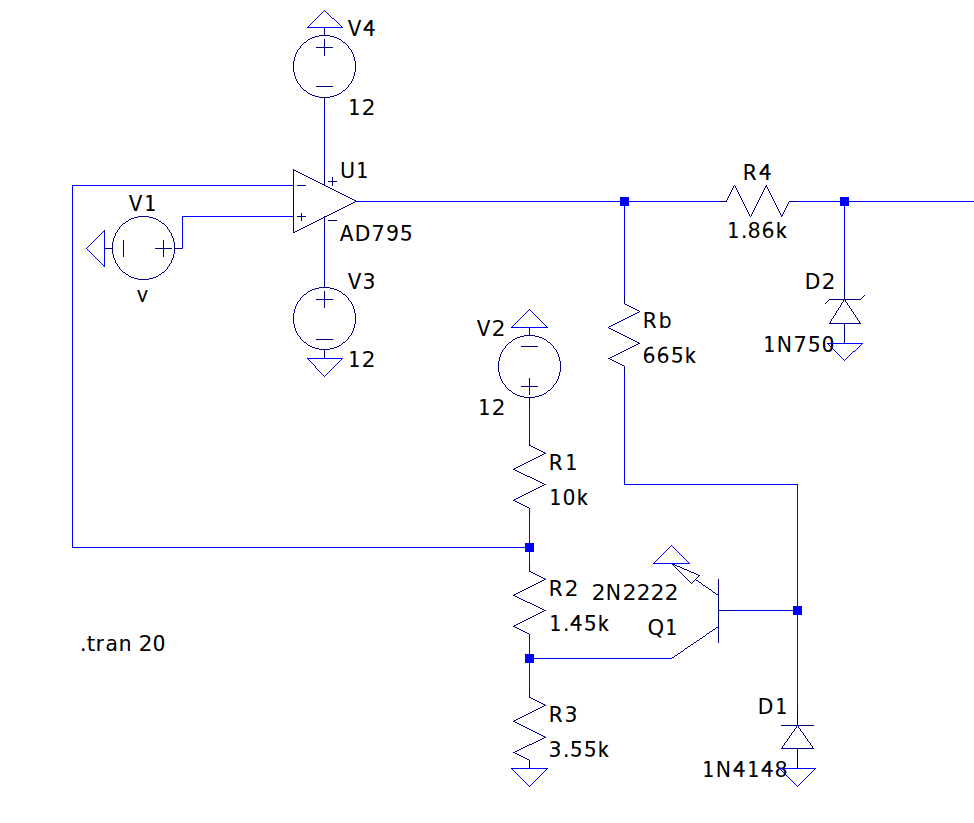
\includegraphics[width=0.7\textwidth]{../images/task5/cheme.png}
	\caption{Триггер Шмитта}
\end{figure}

\begin{figure}[H]
	\centering
	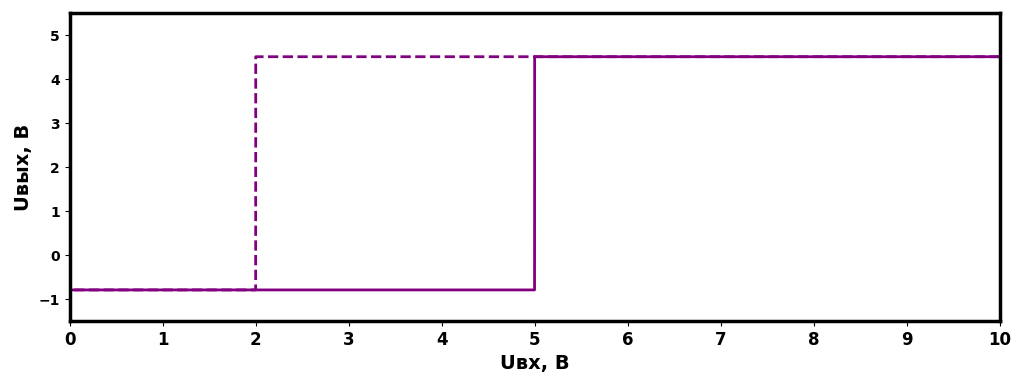
\includegraphics[width=1\textwidth]{../images/task5/grafic.png}
	\caption{Передаточная характеристика $U_{\text{вых}} = f(U_{\text{вх}})$}
\end{figure}

\textbf{Вывод:} триггер переключается в высокий уровень ($\approx 4{,}5$ В)
при $U_{\text{вх}} = U_{\text{ВТО}} = 5$ В и возвращается в низкий уровень
при $U_{\text{вх}} = U_{\text{НТО}} = 2$ В. Ширина гистерезиса составляет
$\Delta U = 3$ В.

\newpage
\section{Исследование компаратора с окном}

Схема компаратора с окном собрана на двух ОУ AD795, питание $\pm 12$ В,
$U_{\text{оп}} = 12$ В, $R_4 = 2$ кОм.

Расчёт делителя при $U_{\text{ВТО}} = 6{,}5$ В, $U_{\text{НТО}} = 4{,}5$ В,
$I_{\text{дел}} = 5$ мА:

\[
R_1 = \frac{U_{\text{оп}} - U_{\text{ВТО}}}{I_{\text{дел}}} = \frac{12 - 6{,}5}{5} = 1{,}1 \text{ кОм}
\]
\[
R_2 = \frac{U_{\text{ВТО}} - U_{\text{НТО}}}{I_{\text{дел}}} = \frac{6{,}5 - 4{,}5}{5} = 0{,}4 \text{ кОм}
\]
\[
R_3 = \frac{U_{\text{НТО}}}{I_{\text{дел}}} = \frac{4{,}5}{5} = 0{,}9 \text{ кОм}
\]


\begin{figure}[H]
	\centering
	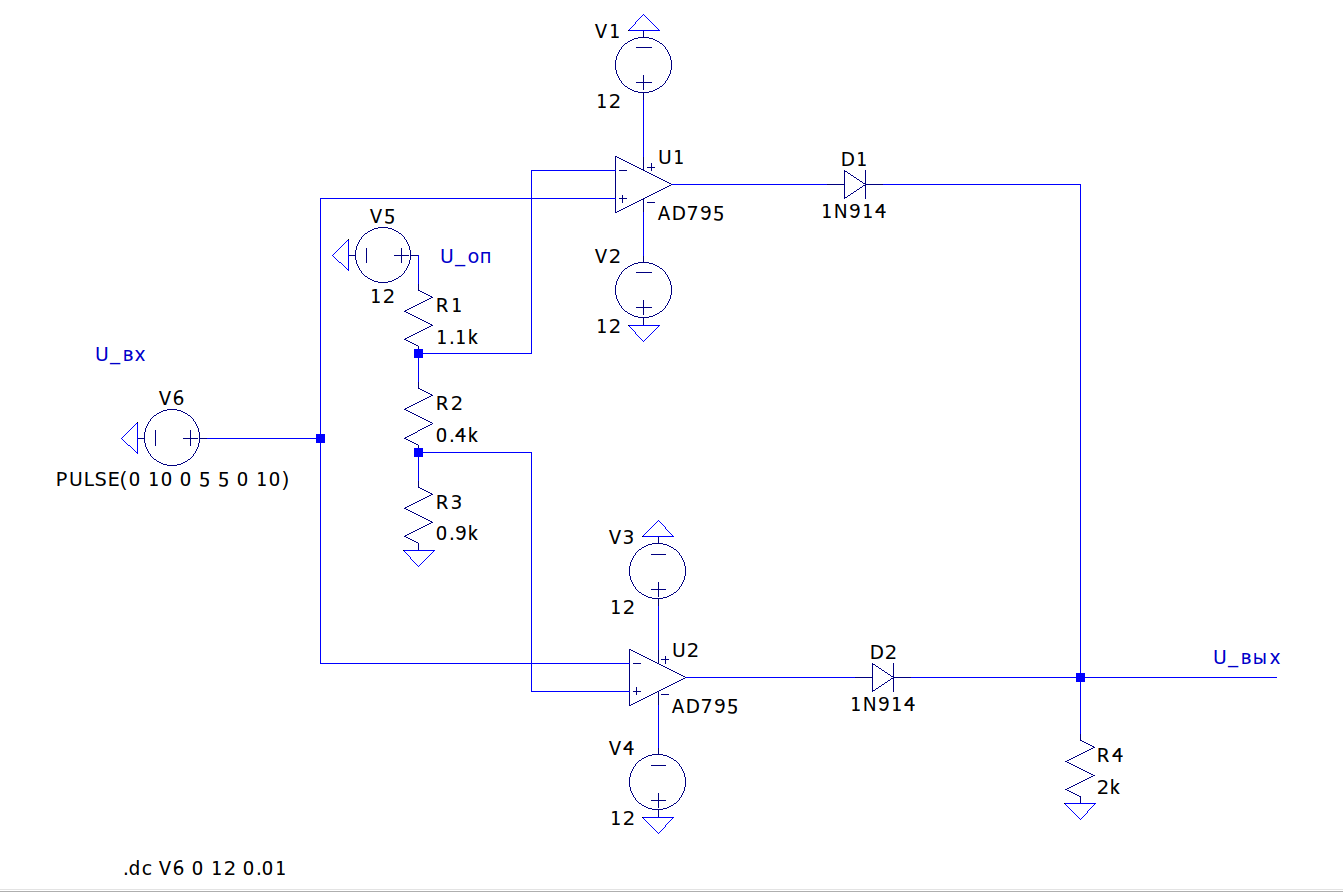
\includegraphics[width=0.8\textwidth]{../images/task6/chema.png}
	\caption{Компаратор с окном}
\end{figure}

\begin{figure}[H]
	\centering
	
\includegraphics[width=1\textwidth]{../images/task6/grafic.png}
	\caption{Передаточная характеристика $U_{\text{вых}} = f(U_{\text{вх}})$}
\end{figure}

\textbf{Вывод:} выход высокий ($\approx 7{,}5$ В) при $U_{\text{вх}}$ вне окна
и низкий ($\approx 0$ В) при $U_{\text{НТО}} < U_{\text{вх}} < U_{\text{ВТО}}$,
то есть в диапазоне от 4{,}5 В до 6{,}5 В.












\end{document}